\documentclass[a0paper,portrait]{baposter}



\usepackage{wrapfig}
\usepackage{lmodern}

\usepackage[utf8]{inputenc} %unicode support
\usepackage[T1]{fontenc}
\usepackage{hyperref}


\selectcolormodel{RGB}

\graphicspath{{figures/}} % Directory in which figures are stored


\newcommand{\compresslist}{%
\setlength{\itemsep}{0pt}%
\setlength{\parskip}{1pt}%
\setlength{\parsep}{0pt}%
}

\newenvironment{boenumerate}
  {\begin{enumerate}\renewcommand\labelenumi{\textbf\theenumi.}}
  {\end{enumerate}}



\begin{document}

\definecolor{loriadark}{RGB}{203,93,155}
\definecolor{loriablue}{RGB}{61,173,226}
\definecolor{loriapink}{RGB}{88,138,181}

\begin{poster}
{
grid=false,
headerborder=open, % Adds a border around the header of content boxes
colspacing=1em, % Column spacing
bgColorOne=white, % Background color for the gradient on the left side of the poster
bgColorTwo=white, % Background color for the gradient on the right side of the poster
borderColor=loriablue, % Border color
headerColorOne=loriapink, % Background color for the header in the content boxes (left side)
headerColorTwo=loriapink, % Background color for the header in the content boxes (right side)
headerFontColor=white, % Text color for the header text in the content boxes
boxColorOne=white, % Background color of the content boxes
textborder=rounded, %rectangle, % Format of the border around content boxes, can be: none, bars, coils, triangles, rectangle, rounded, roundedsmall, roundedright or faded
eyecatcher=false, % Set to false for ignoring the left logo in the title and move the title left
headerheight=0.11\textheight, % Height of the header
headershape=rounded, % Specify the rounded corner in the content box headers, can be: rectangle, small-rounded, roundedright, roundedleft or rounded
headershade=plain,
headerfont=\Large\textsf, % Large, bold and sans serif font in the headers of content boxes
%textfont={\setlength{\parindent}{1.5em}}, % Uncomment for paragraph indentation
linewidth=2pt % Width of the border lines around content boxes
}
{}
%
%----------------------------------------------------------------------------------------
%	TITLE AND AUTHOR NAME
%----------------------------------------------------------------------------------------
%
{\textsf{Controlled Conversational Models through \\ Conversation-Dedicated Ontology}}
{\sf\vspace{0.3em}\\
Barbara Gendron, under the supervision of Mathieu d'Aquin and Gaël Guibon
\vspace{0.1em}\\
\small{Laboratoire Lorrain de Recherche en Informatique et ses Applications (LORIA), Université de Lorraine
\vspace{0.2em}\\
barbara.gendron@loria.fr
}}
{
    \makebox[110pt][l]{
\includegraphics[width=0.15\textwidth]{all-logos.pdf}} 
}%

\headerbox{1. Context}{name=introduction,column=0,row=0, span=3}{
Predicting biological activity of small molecules is a key element of computer-aided drug design.
Existing methods often fail to identify ligands with similar physicochemical properties but different structures.
Many of the current approaches rely on generating 3D conformations, which leads to sampling problems and unacceptably high computational costs for large sets of molecules.
Herein we present DeCAF -- a novel method for describing ligand properties and a fast and effective tool for comparing multiple molecules, and merging them into a single pharmacophore model.
DeCAF is written as an open source Python module (\textbf{\color{loriablue}http://bitbucket.org/marta-sd/decaf}) and can be easily combined with RDKit to facilitate ligand-based drug design.
}


\headerbox{2. Methodology}{name=model,column=0,below=introduction,span=1}{

To describe a molecule, DeCAF substitutes its functional groups with pharmacophoric points (hence the "F" in the algorithm's name).
Points are organised into an undirected graph.
Lengths of the edges in the graph represents the number of bonds between pharmacophoric points.
To describe a molecule, DeCAF substitutes its functional groups with pharmacophoric points (hence the "F" in the algorithm's name).
Points are organised into an undirected graph.
Lengths of the edges in the graph represents the number of bonds between pharmacophoric points.
To describe a molecule, DeCAF substitutes its functional groups with pharmacophoric points (hence the "F" in the algorithm's name).
Points are organised into an undirected graph.
Lengths of the edges in the graph represents the number of bonds between pharmacophoric points.
To describe a molecule, DeCAF substitutes its functional groups with pharmacophoric points (hence the "F" in the algorithm's name).
Points are organised into an undirected graph.
Lengths of the edges in the graph represents the number of bonds between pharmacophoric points.\\
\noindent Some interesting papers:
\begin{itemize}
    \item One
    \item Two
    \item Three
\end{itemize}

\begin{center}
    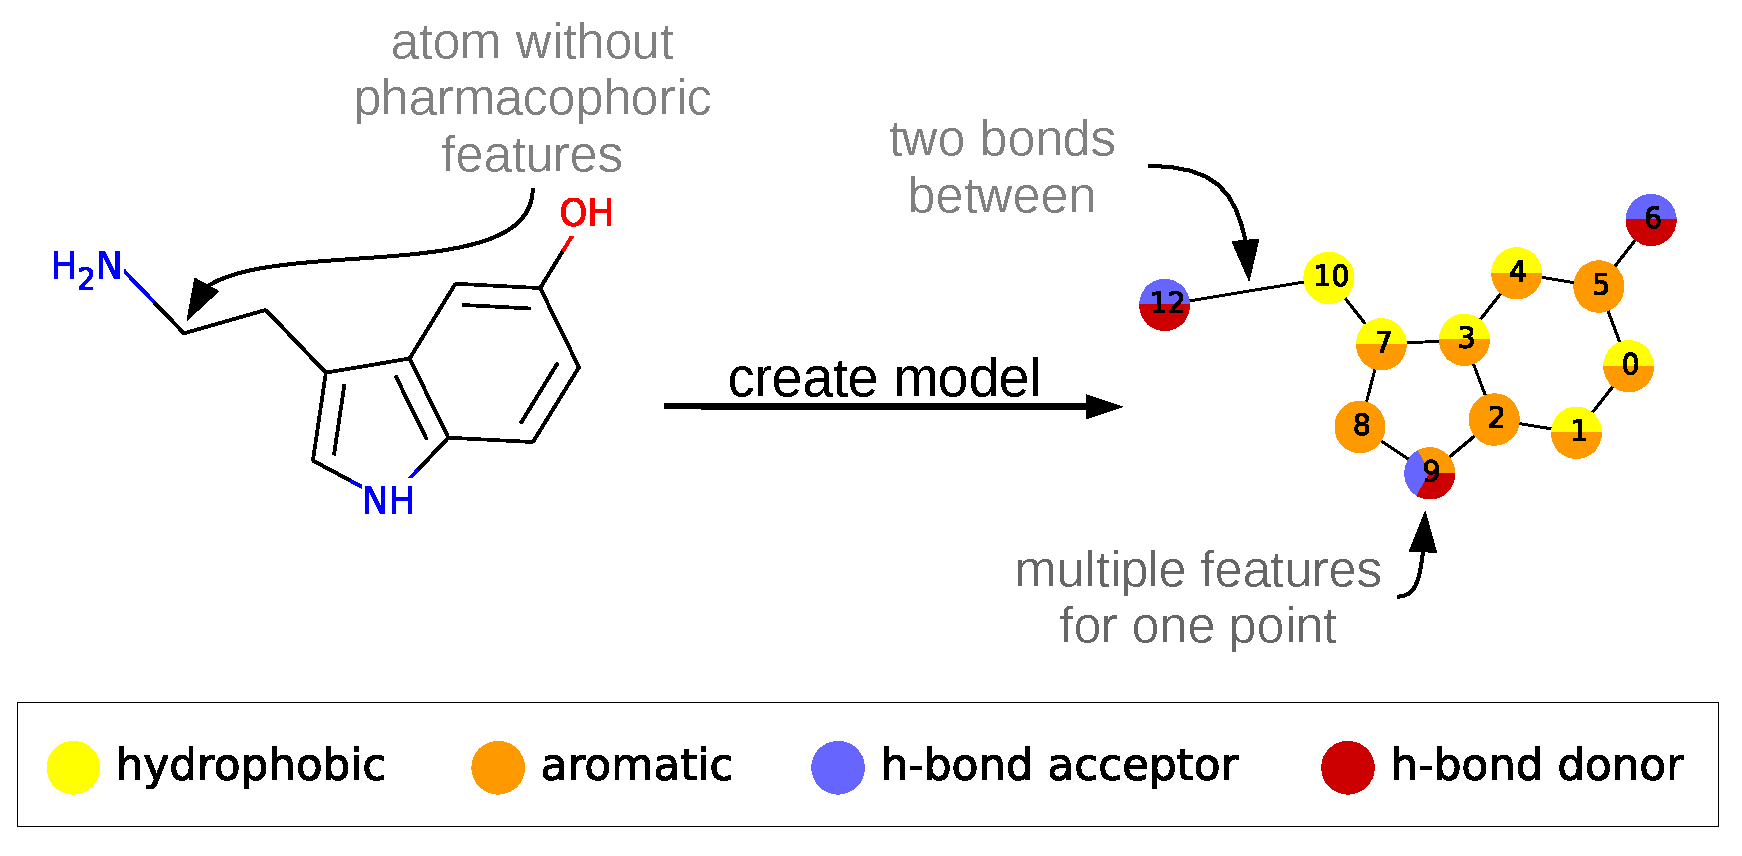
\includegraphics[width=\linewidth]{phar}
\end{center}
%\vspace{-2pt}
}

\headerbox{3. Objectives}{name=screen,span=2,column=1,below=introduction}{ % To reduce this block to 1 column width, remove 'span=2'

\begin{wrapfigure}{l}{0.25\textwidth}
    \vspace{-15pt}
    \begin{center}
        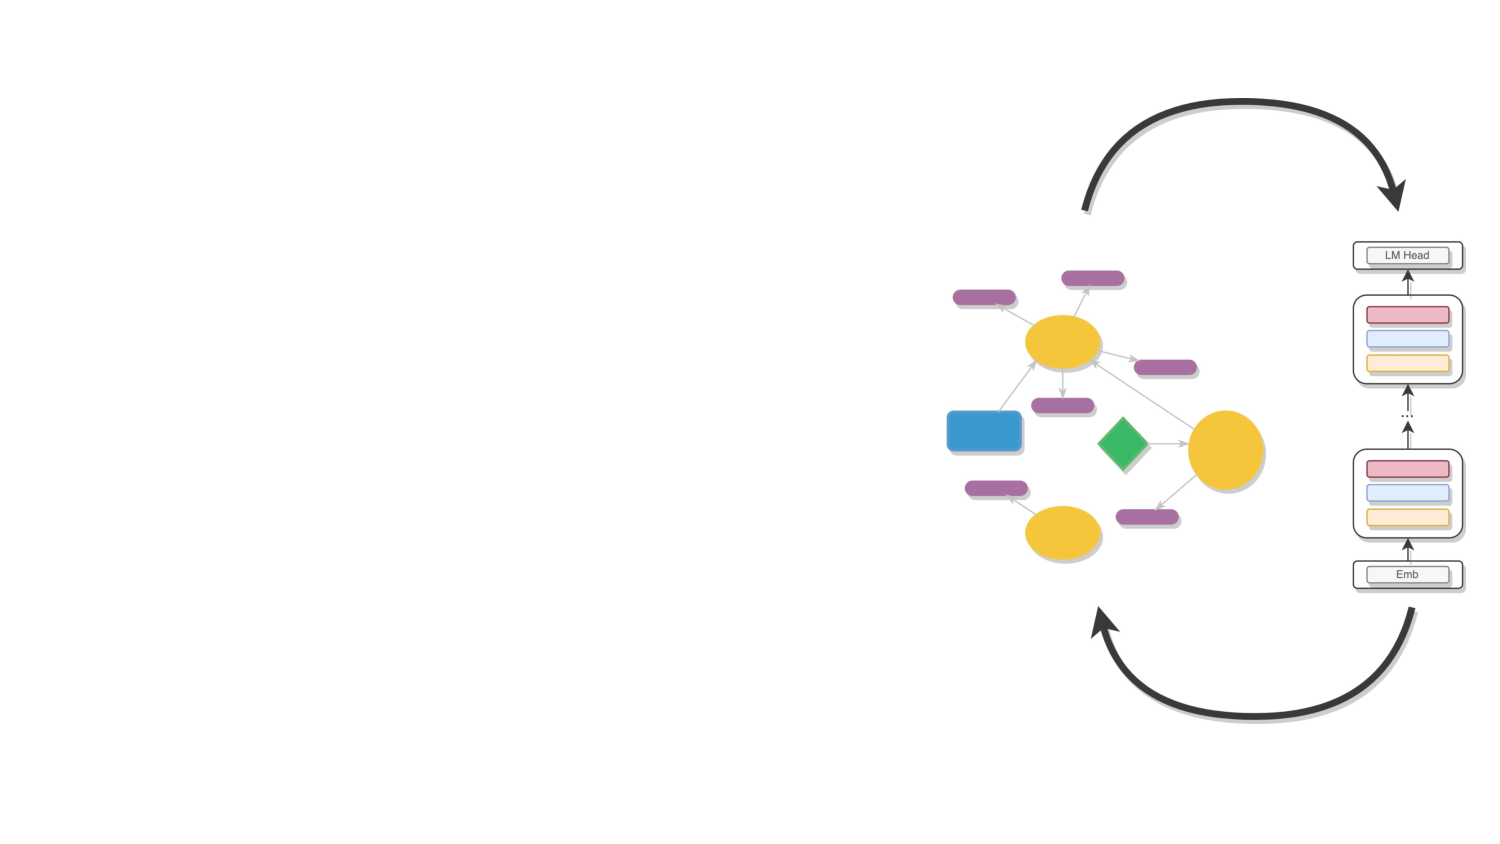
\includegraphics[width=\linewidth]{general-idea.pdf}
    \end{center}
\end{wrapfigure}


We tested DeCAF in 35 diverse targets taken from the DUD-E database, to evaluate its power to classify molecules as active or inactive.
We compared DeCAF to the renowned \textbf{SEA (Similarity Ensemble Approach)} algorithm \cite{keiser2007relating}, which uses Tc as a similarity measure.
Dataset preparation steps are shown on the left diagram.
Comparison results (\textbf{ROC AUC} values for each receptor) are shown below.
% Please ask me about details.
\begin{itemize}
    \item One
    \item Two
    \item Three
\end{itemize}

}


\headerbox{4. OntoGPT: LLM Fine-Tuning Based on Ontology Validation}{name=sea,span=2,column=1,below=screen}{ % To reduce this block to 1 column width, remove 'span=2'
This tool is currently under development...\\
Blablabla

\begin{center}
    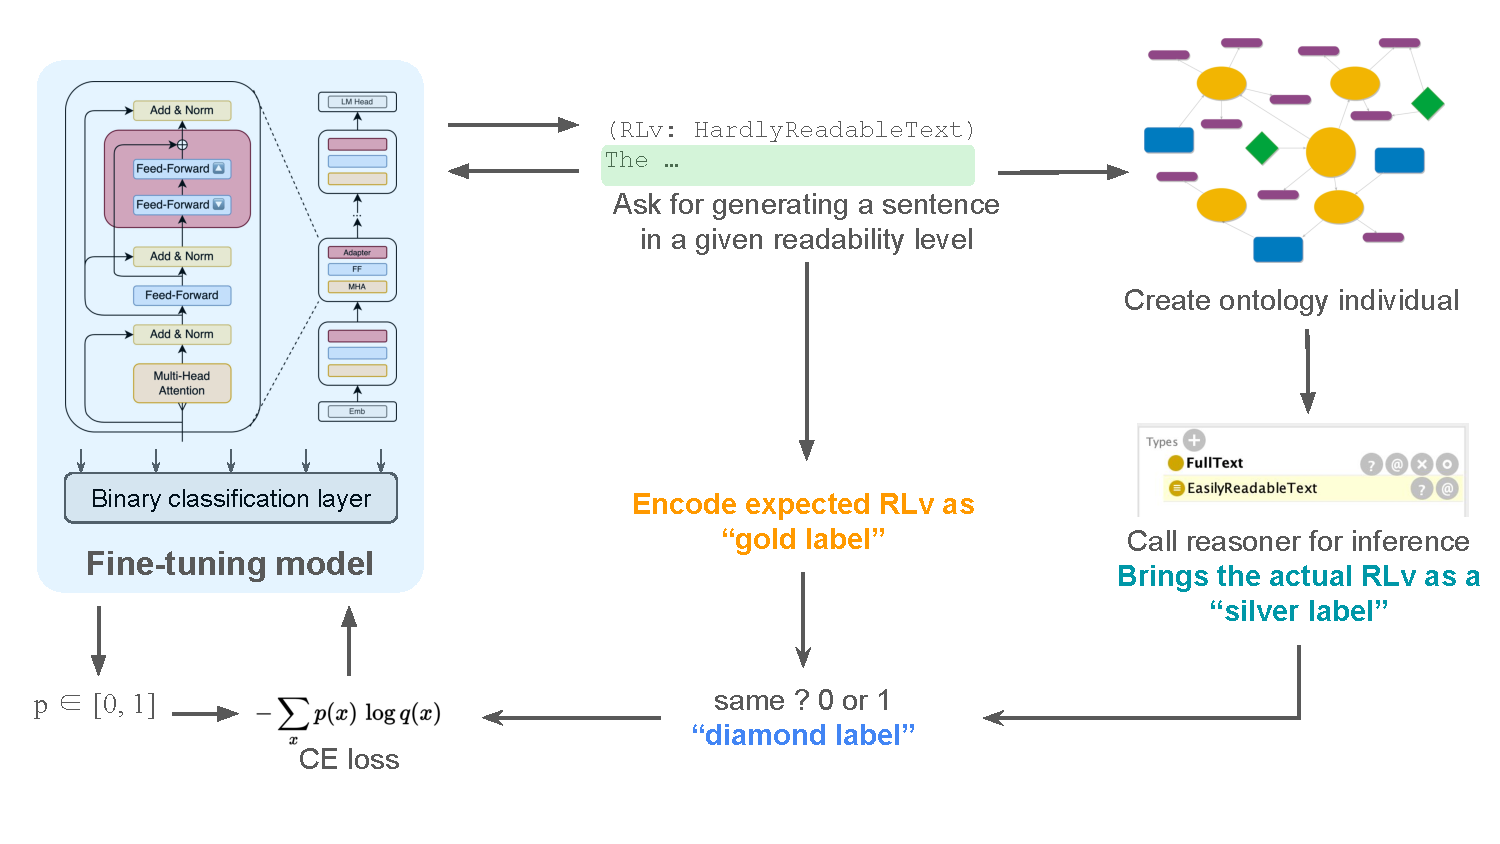
\includegraphics[width=0.95\linewidth]{ft-pipeline.pdf}
\end{center}
}


\headerbox{5. Related Work}{name=conclusion,column=1,below=sea,span=2,above=bottom}{
% DeCAF is a chemoinformatical tool that can be helpful in ligand-based drug design.
% It provides a comprehensive molecule description and a fast algorithms for comparing and aligning multiple ligands.
We proved that DeCAF is a significant improvement over the SEA algorithm, a popular method for comparing sets of ligands.
\begin{boenumerate}\compresslist
    \item DeCAF gives better results for 23 out of 35 receptors.
    \item For targets with easily separable active and inactive datasets, SEA and DeCAF give similar results.
    \item In cases in which SEA fails to identify active molecules, our method performs substantially better.
\end{boenumerate}
% It can be also used in other [procedures], such as database screening or drug repositioning.
% DeCAF is written in Python and freely available at \textbf{\color{loriablue}http://bitbucket.org/marta-sd/decaf}. 
}


\headerbox{6. References}{name=references,column=0,span=1,below=model,above=bottom}{


%\small % Reduce the font size in this block
\renewcommand{\section}[2]{\vskip 0.05em} % Get rid of the default "References" section title
%\nocite{*} % Insert publications even if they are not cited in the poster


\bibliographystyle{unsrt}
\bibliography{poster} % Use sample.bib as the bibliography file
}

\end{poster}

\end{document}
